\usetikzlibrary{arrows}

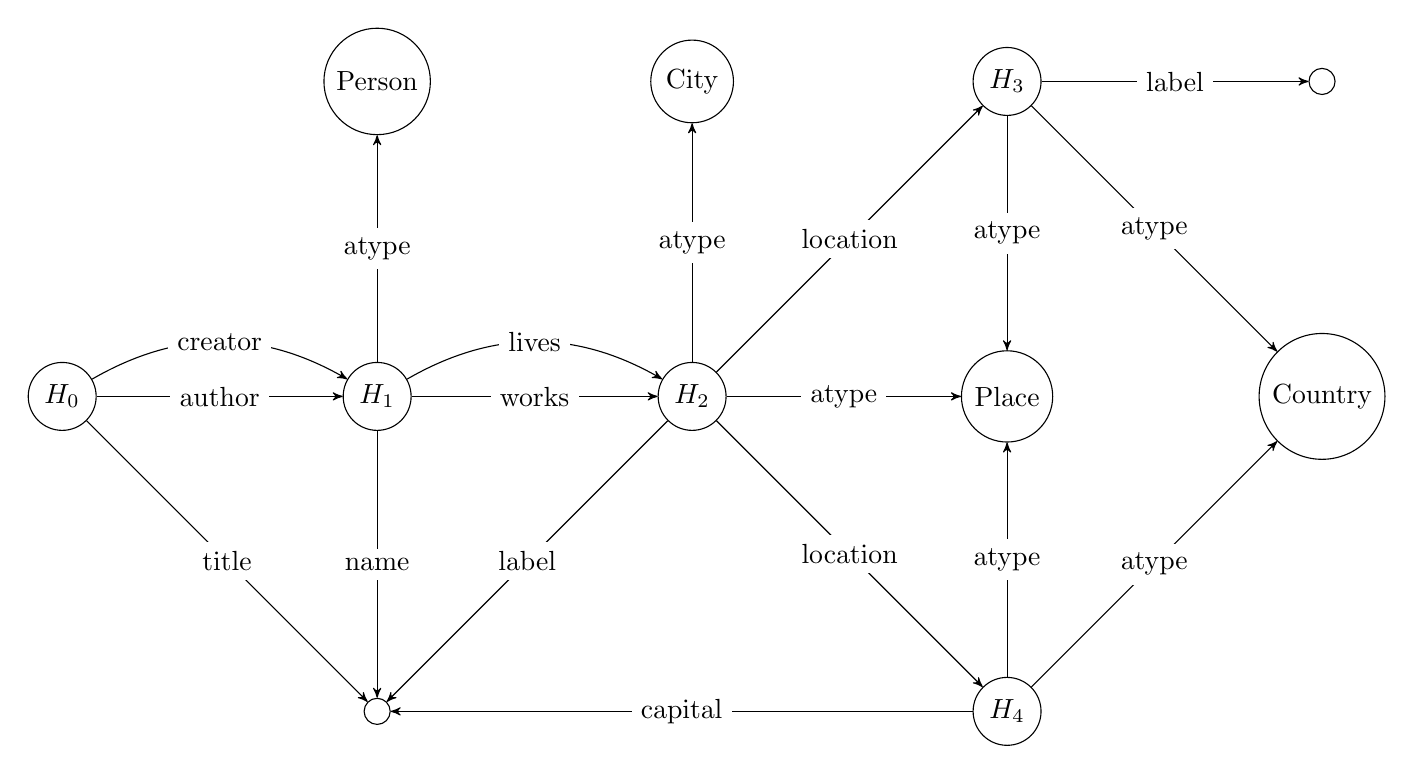
\begin{tikzpicture}[->,>=stealth',node distance=4cm]
\node [draw,circle] (n0) {$H_0$};
% \node (n0) [draw,thick,rectangle,inner sep=0] {
% \begin{tabular}{l}
% \multicolumn{1}{c}{$H_0$} \\
% \hline
% \\
% \hline
% - title
% \end{tabular}
% };

\node [draw,circle,right of = n0] (n1) {$H_1$};
% \node (n1) [draw,thick,rectangle,inner sep=0,right of = n0] {
% \begin{tabular}{l}
% \multicolumn{1}{c}{$H_1$} \\
% \hline
% - Person \\
% \hline
% - name
% \end{tabular}
% };

\node [draw,circle,above of = n1] (person) {Person};
\node [draw,circle,right of = n1] (n2) {$H_2$};
% \node (n2) [draw,thick,rectangle,inner sep=0,right of = n1] {
% \begin{tabular}{l}
% \multicolumn{1}{c}{$H_2$} \\
% \hline
% - City \\
% \hline
% - label
% \end{tabular}
% };

\node [draw,circle,right of = n2] (place) {Place};
\node [draw,circle,above of = place] (n3) {$H_3$};
% \node (n3) [draw,thick,rectangle,inner sep=0,above right of = n2] {
% \begin{tabular}{l}
% \multicolumn{1}{c}{$H_3$} \\
% \hline
% - Place \\
% - Country \\
% \hline
% - label
% \end{tabular}
% };

\node [draw,circle,above of = n2] (city) {City};
\node [draw,circle,below of = place] (n4) {$H_4$};
% \node (n4) [draw,thick,rectangle,inner sep=0,below right of = n2] {
% \begin{tabular}{l}
% \multicolumn{1}{c}{$H_4$} \\
% \hline
% - Place \\
% - Country \\
% \hline
% - capital
% \end{tabular}
% };

\node [draw,circle,right of = place] (country) {Country};
\node [draw,circle,below of = n1] (s1) {$\varnothing$};
\node [draw,circle,right of = n3] (s2) {$\varnothing$};

\path
(n0) edge node[fill=white] {author} (n1)
(n0) edge[bend left] node[fill=white] {creator} (n1)
(n1) edge node[fill=white] {\gls{atype}} (person)
(n1) edge node[fill=white] {works} (n2)
(n1) edge[bend left] node[fill=white] {lives} (n2)
(n2) edge node[fill=white] {\gls{atype}} (city)
(n2) edge node[fill=white] {location} (n3)
(n2) edge node[fill=white] {location} (n4)
(n2) edge node[fill=white] {\gls{atype}} (place)
(n3) edge node[fill=white] {\gls{atype}} (country)
(n4) edge node[fill=white] {\gls{atype}} (country)
(n3) edge node[fill=white] {\gls{atype}} (place)
(n4) edge node[fill=white] {\gls{atype}} (place)
(n0) edge node[fill=white] {title} (s1)
(n1) edge node[fill=white] {name} (s1)
(n2) edge node[fill=white] {label} (s1)
(n4) edge node[fill=white] {capital} (s1)
(n3) edge node[fill=white] {label} (s2)
;
\end{tikzpicture}